
\section{Experiments}
\label{sec:experiments}

\subsection{Experimental Setup}
\label{sec:exp_setup}

\paragraph{Base model and evaluation.}
We evaluate on DeepSeek-R1-Distill-Qwen-7B~\citep{deepseek2025r1}, a 7B-parameter reasoning model built on the Qwen2.5 architecture~\citep{qwen2.5} with GQA~\citep{ainslie2023gqa} (architecture details in Section~\ref{sec:prelim}).
We evaluate on GSM8K~\citep{cobbe2021gsm8k}, a benchmark of 1{,}319 grade-school math problems requiring multi-step arithmetic reasoning.
We report exact-match accuracy: the final numerical answer is extracted from the model's generation and compared against the ground truth.
For rapid iteration during development, we use a 100-problem subset ($N{=}100$); final results use the full test set ($N{=}1{,}319$).
The original unpruned model achieves 90.83\% on GSM8K (greedy decoding).

\paragraph{Pruning methods.}
We compare four pruning criteria at 20\% structured sparsity, all removing the same number of MLP channel groups (200 of 784 across 28 layers, ${\sim}$1.45B parameters) with identical per-layer capacity floors (${\ge}$40\% retention per layer):
\begin{enumerate}[nosep,leftmargin=*]
    \item \textbf{CKA-only}: structures ranked by functional overlap $F(h)$ alone (Eq.~\ref{eq:overlap}); the most redundant groups are removed regardless of gradient importance.
    \item \textbf{Random}: uniform random selection among eligible groups.
    \item \textbf{Standard}: Taylor-expansion importance $I(h)$ alone (Eq.~\ref{eq:importance}); the least important groups are removed, following LLM-Pruner~\citep{llmpruner2023}.
    \item \textbf{\rasp{}} ($\alpha{=}1.0$): the composite score $S(h) = I(h) \times (1 - F(h))^\alpha$ (Eq.~\ref{eq:score}), removing structures that are both low-importance and functionally redundant.
\end{enumerate}

\paragraph{Recovery pipeline and hardware.}
All four methods undergo matched two-stage recovery.
Stage~1 (SFT warmup): 2 epochs on 7{,}473 GSM8K chain-of-thought examples with teacher forcing (37 minutes), restoring EOS generation and basic format compliance.
Stage~2 (GRPO): Group Relative Policy Optimization~\citep{shao2024grpo} with learning rate $1{\times}10^{-6}$, maximum completion length 1{,}024 tokens, KL penalty coefficient $\beta{=}0.01$, sampling temperature 0.4, DAPO-style clipped loss, and binary reward ($r{=}1$ if correct, $r{=}0$ otherwise), trained for 100 steps on 1{,}000 GSM8K training problems.
All methods share identical GRPO hyperparameters, including \texttt{reward\_desert\_patience}{$=$}50.
Seeds vary at the GRPO stage; pruning calibration and SFT use identical configurations across all methods.
We repeat GRPO training with 3 random seeds for CKA-only and Standard (Table~\ref{tab:decoupling}).
CKA-only achieves 64.39\% $\pm$ 0.19\,pp (std across seeds), Standard 59.84\% $\pm$ 0.38\,pp; the 4.55\,pp gap is robust across seeds (Welch's $t$-test, $p{=}0.0009$, Cohen's $d{=}11.1$; 95\% CI for mean difference: $[3.62, 5.47]$\,pp), confirming that recovery capacity differences are structural rather than stochastic.
All experiments run on 2$\times$ NVIDIA RTX PRO 6000 GPUs (94\,GB VRAM each); pruning variants are trained in parallel on separate GPUs under identical wall-clock conditions.


\subsection{Recovery Capacity Spectrum}
\label{sec:recovery_gradient}

\begin{table}[t]
\centering
\small
\caption{Recovery capacity spectrum: GRPO dynamics for four pruning criteria at 20\% sparsity under identical configuration (lr $1{\times}10^{-6}$, $\beta{=}0.01$, $T{=}0.4$, 100 steps). Peak reward = best across 100 training steps. $f_0$: fraction of training batches where all sampled completions receive identical reward (lower = healthier exploration). Best in \textbf{bold}, second-best \underline{underlined}.}
\label{tab:recovery_gradient}
\begin{tabular}{@{}lcccc@{}}
\toprule
Method & Peak Rew.\,$\uparrow$ & Mean Rew.\,$\uparrow$ & Min $f_0$\,$\downarrow$ & Behavior \\
\midrule
CKA-only & \textbf{0.354} & \textbf{0.285} & \textbf{0.125} & Active learning \\
Random$^\ddagger$ & \underline{0.190} & \underline{0.164} & \underline{0.300} & Stagnation \\
Standard & 0.081 & 0.050 & 0.500 & Borderline collapse \\
\rasp{}$^\ddagger$ & 0.061 & 0.031 & 0.675 & Full collapse \\
\bottomrule
\multicolumn{5}{l}{\footnotesize $^\ddagger$Single seed ($N{=}1$). CKA-only and Standard validated with 3 seeds (Table~\ref{tab:decoupling}).}
\end{tabular}
\end{table}


\begin{figure}[t]
    \centering
    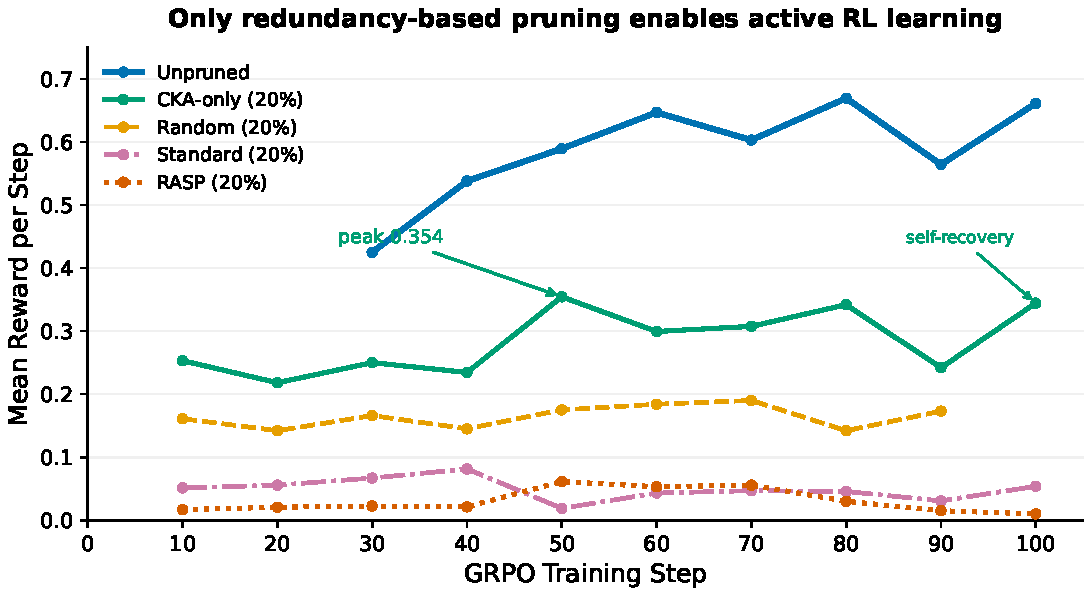
\includegraphics[width=\columnwidth]{figures/paper/fig2_reward_trajectories.pdf}
    \caption{GRPO reward trajectories for four pruning criteria and the unpruned model under identical training configuration ($\beta{=}0.01$, $T{=}0.4$, 100 steps). CKA-only reaches 0.354 peak reward with an observed recovery event at step 90. Random oscillates between 0.14 and 0.19 (training timed out at step 97; 9 steps shown). Standard peaks at 0.081 before borderline collapse. \rasp{} peaks at 0.061 (step 50) and declines to 0.010 by step 100.}
    \label{fig:reward_trajectories}
\end{figure}

The central finding of this work is that the pruning criterion can significantly influence post-RLVR recovery capacity in our experimental setting.
Under controlled GRPO training with identical hyperparameters, the four pruning methods produce qualitatively distinct training dynamics that form a clear recovery capacity spectrum: CKA-only $\gg$ Random $\gg$ Standard $>$ \rasp{}.
Table~\ref{tab:recovery_gradient} summarizes the key metrics, and Figure~\ref{fig:reward_trajectories} shows the reward trajectories over 100 GRPO steps.

\begin{figure}[t]
    \centering
    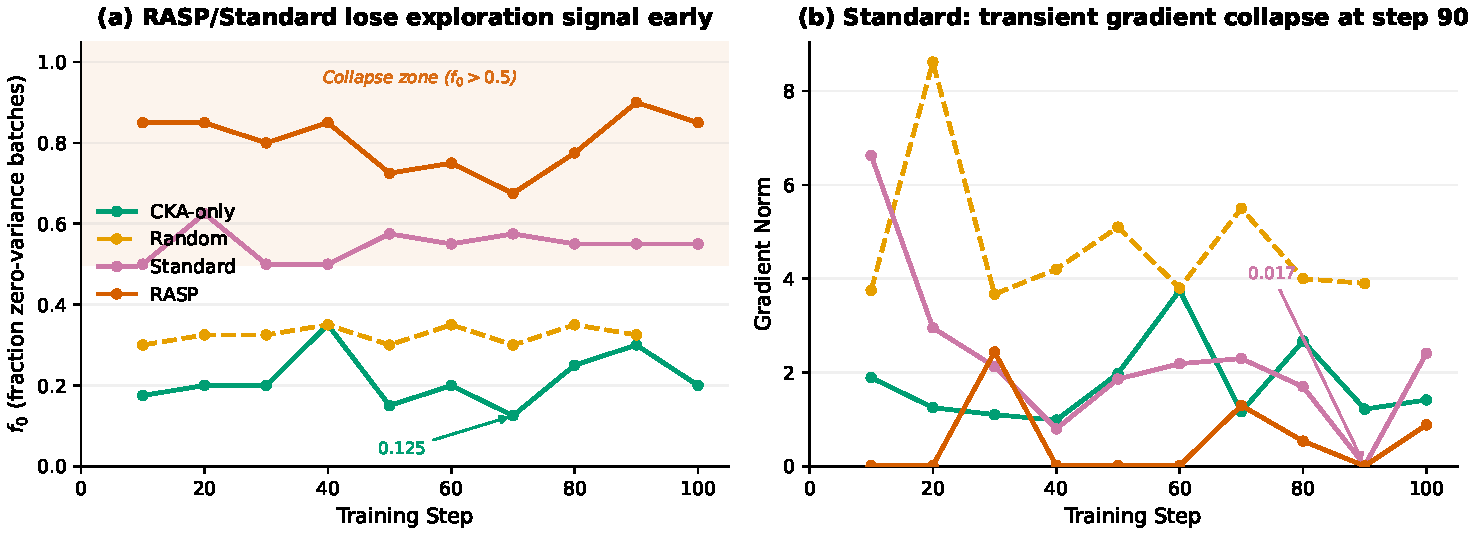
\includegraphics[width=\columnwidth]{figures/paper/fig3_collapse_dynamics.pdf}
    \caption{Training dynamics diagnostics. (a)~$f_0$ (fraction of zero-variance batches): CKA-only stays below 0.35; Standard and \rasp{} remain in the collapse zone ($f_0 > 0.5$) throughout training. (b)~Gradient norm: Standard exhibits a transient minimum of 0.017 at step 90 before recovering to 2.41 at step 100; \rasp{} gradient norms remain predominantly near zero.}
    \label{fig:collapse_dynamics}
\end{figure}

CKA-only pruning is the only method that produces active learning under GRPO.
Reward reaches a peak of 0.354 (mean 0.285) with $f_0$ as low as 0.125, including a recovery event at step 90 where reward rebounds from a transient perturbation.
Random pruning produces stagnation: reward oscillates between 0.142 and 0.190 with $f_0$ near 0.33.

Standard pruning exhibits borderline collapse (Figure~\ref{fig:collapse_dynamics}): reward peaks at 0.081 (step 40) then oscillates near 0.05, with $f_0 \geq 0.500$ throughout---more than half of batches produce no learning signal.
\rasp{} produces full collapse: reward peaks at 0.061 (step 50) then declines to 0.010 by step 100, with $f_0 > 0.675$ and clipped ratio $>$ 90\%.

The 5.8$\times$ peak reward gap (CKA-only 0.354 vs \rasp{} 0.061) arises from models pruned to identical parameter budgets with identical GRPO configurations; the only variable is which structures were removed.


\subsection{Reward-Accuracy Decoupling}
\label{sec:decoupling}

\begin{table}[t]
\centering
\small
\caption{GRPO responsiveness on GSM8K ($N{=}1{,}319$, greedy decoding). All pruned models use the controlled v5 GRPO configuration (identical hyperparameters including \texttt{reward\_desert\_patience}{$=$}50), evaluated at step 100. CKA-only and Standard report mean $\pm$ std over 3 GRPO seeds; \rasp{} uses a single seed. Best in \textbf{bold}, second-best \underline{underlined}.}
\label{tab:decoupling}
\begin{tabular}{@{}lcccc@{}}
\toprule
Model & SFT Acc.\,(\%) & GRPO Acc.\,(\%) & $\Delta$\,(pp) & Peak Rew. \\
\midrule
Unpruned & \textbf{81.27} & \textbf{81.27} & $\phantom{-}$0.00 & \textbf{0.669} \\
CKA-only 20\% & \underline{63.91} & \underline{64.39{\scriptsize$\pm$0.19}} & $+$0.48 & \underline{0.354} \\
Standard 20\% & 59.29 & 59.84{\scriptsize$\pm$0.38} & $+$0.55 & 0.081 \\
\rasp{} 20\% & 61.49 & 60.88 & $-$0.61 & 0.061 \\
Random 20\%$^\ddagger$ & -- & -- & -- & 0.190 \\
\midrule
ShortGPT 20\%$^\dagger$ & 44.73 & 43.37 & $-$1.36 & -- \\
\bottomrule
\multicolumn{5}{l}{\footnotesize $^\dagger$Depth pruning baseline~\citep{shortgpt2024}; removes entire layers.} \\
\multicolumn{5}{l}{\footnotesize $^\ddagger$Accuracy not evaluated; checkpoint not preserved.}
\end{tabular}
\end{table}


GRPO reward trajectory reflects training capacity---the model's ability to learn from RL signal---not downstream accuracy.
At 20\% sparsity, accuracy changes are small across all pruned methods ($|\Delta| < 1$\,pp: CKA-only $+$0.48, Standard $+$0.55, \rasp{} $-$0.61\,pp; Table~\ref{tab:decoupling}) despite the 4.4$\times$ peak reward gap.

The degree of decoupling varies with sparsity.
At 15\% (3-seed GRPO), SFT establishes a 5.69\,pp gap between CKA-only and Standard (72.18\% vs 66.49\%; single SFT seed), which GRPO maintains or slightly amplifies to 7.20\,pp (72.76\% vs 65.56\%; Welch's $t$-test, $p{<}0.001$).
At 20\%, the differential GRPO contribution is negligible: SFT establishes a 4.62\,pp gap that GRPO preserves (4.55\,pp).
At 25\% (single seed), decoupling is most extreme: Standard's peak reward collapses to 0.008 yet accuracy changes by only $+$0.99\,pp (Appendix~\ref{sec:appendix_cross_sparsity}).
Across all four fine-grained pruning criteria and both sparsity levels tested (20\% and 25\%), $|\Delta| < 1$\,pp without exception on GSM8K (Tables~\ref{tab:decoupling},~\ref{tab:cross_sparsity}), extending to MATH-500 where all completed SFT/GRPO pairs show $|\Delta| \leq 1.2$\,pp (Appendix~\ref{sec:appendix_math500}).
This pattern suggests that moderate structural damage (15\%) preserves enough capacity for GRPO to differentially benefit CKA-only pruning, while more aggressive pruning (20--25\%) exceeds the threshold where GRPO can improve upon SFT baselines.

Extended training to 300 steps at 20\% confirms: accuracy remains unchanged (CKA-only 64.37\%$\to$64.37\%, Standard 59.44\%$\to$59.29\%; single seed).
The pruning-criterion ranking transfers to MATH-500~\citep{hendrycks2021math} (CKA-only 26.6\% vs Standard 25.8\% vs \rasp{} 22.6\%; Appendix~\ref{sec:appendix_math500}), and decoupling holds across HumanEval~\citep{chen2021humaneval} and MBPP~\citep{austin2021mbpp} (all pruned-model GRPO $|\Delta| < 2$\,pp; Appendix~\ref{sec:appendix_mbpp}).
\label{sec:ood}
ShortGPT~\citep{shortgpt2024} depth pruning is the exception: GRPO interaction is task-dependent ($-$1.36\,pp on GSM8K, $+$4.01\,pp on MBPP; Tables~\ref{tab:decoupling},~\ref{tab:mbpp}), unlike the uniformly neutral deltas of fine-grained methods ($|\Delta| \leq 1.34$\,pp).


\subsection{Additional Results}
\label{sec:additional_results}

\paragraph{Post-SFT accuracy does not predict GRPO outcome.}
\label{sec:sft_gradient}
Under SFT alone, CKA-only (63.91\%) $>$ \rasp{} (61.49\%) $>$ Standard (59.29\%), yet under GRPO the \rasp{}/Standard ordering reverses (peak 0.081 vs 0.061).
More strikingly, ShortGPT post-SFT (44.73\%) shows GRPO actively harming accuracy ($-$1.36\,pp), while unstructured pruning achieves the highest post-SFT accuracy (87.87\%) with GRPO accuracy 87.64\% ($\Delta{=}{-}0.23$\,pp), confirming that pruning criteria are irrelevant when structural damage is minimal (96.5\% dense retention).
Post-SFT accuracy does not monotonically determine GRPO recovery outcome; the recovery capacity spectrum is driven by structural properties of the pruned architecture, not residual SFT quality.

\paragraph{Additional results.}
\label{sec:sparsity_cliff}
All methods collapse at 30\% sparsity, validating 20\% as the operating point (Appendix~\ref{sec:appendix_sparsity_cliff}).
Pruning reduces parameters by 19\% and memory by ${\sim}$28\% (Appendix~\ref{sec:appendix_inference}).
The CKA coefficient $\alpha$ shows a non-monotonic pattern in post-prune accuracy across $\{0.0, 0.25, 0.5, 1.0, 2.0, 4.0\}$; notably, $\alpha{=}4.0$ exhibits active GRPO learning (peak reward 0.256) with preliminary accuracy 62.93\%, contrasting with $\alpha{=}1.0$'s collapse (peak reward 0.061), consistent with CKA dominance driving recovery capacity (Appendix~\ref{sec:appendix_alpha}).\footnote{$\alpha{=}4.0$ results are preliminary ($N{=}774/1{,}319$ samples evaluated); full evaluation pending.}


\subsection{Extended Analysis}
\label{sec:extended_analysis}

\begin{figure}[t]
    \centering
    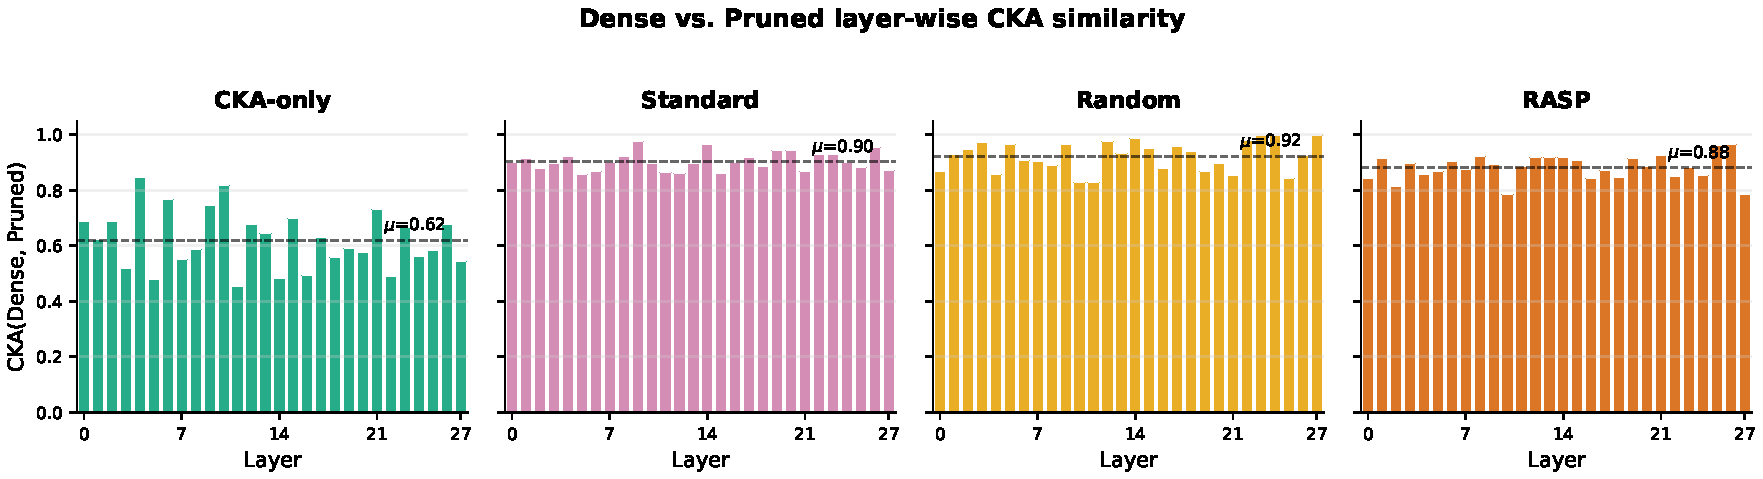
\includegraphics[width=\columnwidth]{figures/paper/fig4_cka_heatmap.pdf}
    \caption{Layer-wise CKA similarity between dense and pruned representations (28 layers). CKA-only diverges most from dense ($\mu{=}0.62$) yet recovers best; Standard ($\mu{=}0.90$), Random ($\mu{=}0.92$), and \rasp{} ($\mu{=}0.88$) preserve dense fidelity but collapse under RL.}
    \label{fig:cka_heatmap}
\end{figure}

\begin{table}[t]
\centering
\small
\caption{Cross-scale validation at 20\% sparsity. 7B: DeepSeek-R1-Distill-Qwen-7B (GSM8K mean over 3 seeds for CKA-only and Standard; see Table~\ref{tab:decoupling}). 1.5B: DeepSeek-R1-Distill-Qwen-1.5B (single seed). GSM8K accuracy ($N{=}1{,}319$). 7B reward = peak across 100 GRPO steps (cf.\ Table~\ref{tab:recovery_gradient}); 1.5B reward = mean across training steps.}
\label{tab:cross_scale}
\begin{tabular}{@{}lcccc@{}}
\toprule
\multirow{2}{*}{Method} & \multicolumn{2}{c}{7B} & \multicolumn{2}{c}{1.5B} \\
\cmidrule(lr){2-3} \cmidrule(lr){4-5}
 & Peak Rew. & GSM8K\,(\%) & Rew. & GSM8K\,(\%) \\
\midrule
CKA-only & \textbf{0.354} & \textbf{64.39} & \textbf{0.238} & \textbf{35.48} \\
Standard & 0.081 & 59.84 & 0.084 & 22.29 \\
\rasp{} & 0.061 & 60.88 & 0.099 & 26.16 \\
Random & 0.190 & -- & -- & -- \\
\bottomrule
\end{tabular}
\end{table}


\paragraph{Representational diversity.}
CKA similarity between dense and pruned representations (Figure~\ref{fig:cka_heatmap}) shows CKA-only diverges most from the dense model ($\mu{=}0.62$), while Standard ($\mu{=}0.90$), Random ($\mu{=}0.92$), and \rasp{} ($\mu{=}0.88$) cluster near 1.0.
Gradient importance preserves dense fidelity at the cost of redundant representations that provide no exploration benefit during GRPO.
Structural overlap analysis reveals that CKA-only concentrates pruning in early layers (L0--9, 72.5\% of removed groups) while preserving later layers critical for reasoning (L16--27), whereas Standard prunes uniformly across depth, removing many late-layer structures that CKA identifies as representationally unique (Appendix~\ref{sec:appendix_overlap}).

\paragraph{Extended training cannot rescue collapse.}
Extending GRPO from 100 to 300 steps (Figure~\ref{fig:extended_training}, Appendix~\ref{sec:appendix_extended}), Standard shows zero net improvement (reward 0.054--0.058, $f_0 > 0.5$ throughout), while CKA-only sustains a 5.5$\times$ gap (0.308 vs 0.056 at step 300). The gap is structural, not a matter of training budget.

\paragraph{Cross-scale and cross-architecture generalization.}
On DeepSeek-R1-Distill-Qwen-1.5B at 20\% sparsity (Table~\ref{tab:cross_scale}), the three-method ordering is preserved (CKA-only 35.48\% $\gg$ \rasp{} 26.16\% $>$ Standard 22.29\%), with reward-accuracy decoupling confirmed at this scale ($|\Delta| < 1$\,pp: CKA-only $-$0.15, Standard $-$0.61\,pp).
To test cross-architecture generalization, we apply CKA-only and Standard pruning to Qwen2.5-Math-7B~\citep{qwen2.5} at 20\% sparsity (Table~\ref{tab:cross_arch}, Appendix~\ref{sec:appendix_cross_arch}).
CKA-only causes near-total initial damage (1.0\% post-prune accuracy vs Standard's 18.5\%), yet SFT recovers CKA-only to 51.50\% $\pm$ 3.53 while Standard remains at 21.00\% $\pm$ 2.88 ($N{=}200$).
This post-prune accuracy reversal---where the method with lower initial accuracy achieves dramatically higher recovery---provides additional evidence that recoverability is shaped by preserved network structure, not starting accuracy.
Cross-architecture validation covers the SFT recovery stage; GRPO validation on Qwen2.5-Math-7B is deferred to future work.


